\documentclass[10pt,a4paper]{article}
\usepackage[latin1]{inputenc}
\usepackage[english]{babel}
\usepackage{amsmath}
\usepackage{amsfonts}
\usepackage{amssymb}
\usepackage{graphicx}
\usepackage{soul}
\usepackage{tikz}

%\documentclass[tikz,border=10pt]{standalone}
\usetikzlibrary{arrows,automata,positioning}
\tikzset{main node/.style={circle,fill=blue!20,draw,minimum size=1cm,inner sep=0pt},}


\begin{document}
\hspace{-2.5cm}\resizebox{12cm}{!}{%
  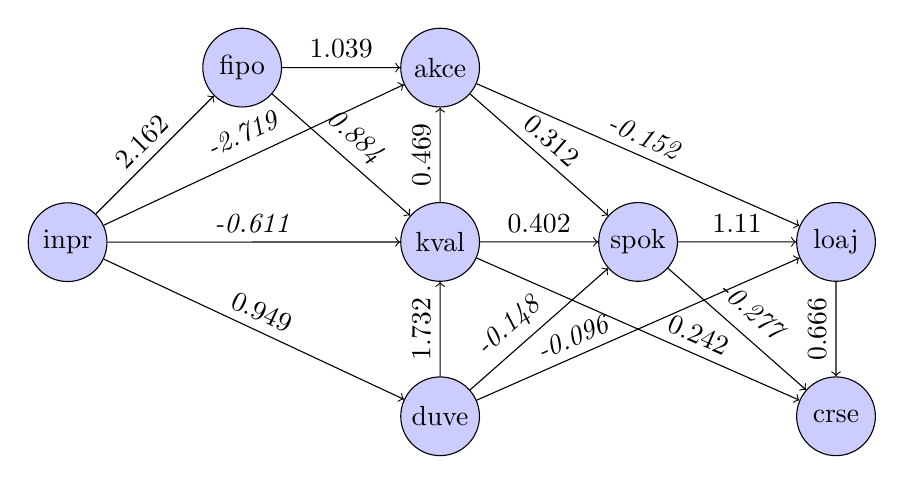
\begin{tikzpicture}[scale=3]
    \node[main node] (1) {inpr};
    \node[main node] (2) [above right = 1.5 cm and 1.5cm of 1]  {fipo};
    \node[main node] (3) [right = 4cm and 1.5cm of 2] {akce};
    \node[main node] (4) [below = 1.2cm and 1.5cm of 3] {kval};
    \node[main node] (5) [below = 1.2cm and 1.5cm of 4] {duve};
    \node[main node] (6) [right = 1.5cm and 1.5cm of 4] {spok};
    \node[main node] (7) [right = 1.5cm and 1.5cm of 6] {loaj};
    \node[main node] (8) [below = 1.2cm and 1.5cm of 7] {crse};

    \path[every node/.style={sloped, anchor=south,auto=false}, ->]
	(1) edge node {$2.162$} (2)
	(1) edge node {\textit{-0.611}} (4) 
	(1) edge node {\textit{-2.719}} (3) 
	(1) edge node {$0.949$} (5) 
	(2) edge node {$1.039$} (3) 
	(2) edge node {\textit{0.884}}  (4) 
	(5) edge node {$1.732$} (4)
	(3) edge node {$0.312$} (6)
	(4) edge node {$0.469$} (3) 
	(5) edge node {\textit{-0.148}$\;\;\;\;\;$} (6) 
	(4) edge node {$0.402$} (6) 
	(6) edge node {$1.11$} (7)  
	(3) edge node {\textit{-0.152} } (7)  
	(5) edge node {\textit{-0.096}$\;\;\;\;\;\;\;\;\;\;\;\;\;\;\;\;$ } (7) 
	(4) edge node {$\;\;\;\;\;\;\;\;\;\;\;\;\;\;\;0.242$} (8) 
	(6) edge node {\textit{-0.277} } (8) 
	(7) edge node {$0.666$} (8) ;
    %%
%    \begin{scope}[xshift=4cm]
%    \node[main node] (1) {};
%    \node[main node] (2) [right = 2cm  of 1]  {$2$}; 
%    \node[main node] (3) [below = 2cm  of 1] {$3$};
%    \node[main node] (4) [right = 2cm  of 3] {$4$};
%
%    \path[draw,thick]
%    (1) edge node {$f(x)=x^2$} (2)
%    (1) edge node {} (4)
%    (3) edge node {} (2)
%    (3) edge node {} (4)
%    ;
%    \end{scope}
\end{tikzpicture}
}
\bigskip

% Table generated by Excel2LaTeX from sheet 'List1'
\begin{table}[htbp]
  \centering
  \caption{Estimates of path coefficients between endogenous constructs.}
    \begin{tabular}{rrrrrr}
      Dependent    &  Independent      & Estimate & Std.err & Z-value & P($>\vert z\vert$) \\
      fipo ~ & inpr  & 2.162 & 0.389 & 5.555 & 0 \\
      kval ~ & inpr  & -0.611 & 0.847 & -0.722 & 0.47 \\
      akce ~ & inpr  & -2.719 & 1.496 & -1.817 & 0.069 \\
      duve ~ & inpr  & 0.949 & 0.128 & 7.41  & 0 \\
      akce ~ & fipo  & 1.039 & 0.497 & 2.091 & 0.036 \\
      kval ~ & fipo  & 0.884 & 0.46  & 1.921 & 0.055 \\
      kval ~ & duve  & 1.732 & 0.728 & 2.381 & 0.017 \\
      spok ~ & akce  & 0.312 & 0.124 & 2.522 & 0.012 \\
      akce ~ & kval  & 0.469 & 0.237 & 1.979 & 0.048 \\
      spok ~ & duve  & -0.148 & 0.261 & -0.566 & 0.572 \\
      spok ~ & kval  & 0.402 & 0.164 & 2.457 & 0.014 \\
      loaj ~ & spok  & 1.11  & 0.223 & 4.973 & 0 \\
      loaj ~ & akce  & -0.152 & 0.111 & -1.365 & 0.172 \\
      loaj ~ & duve  & -0.096 & 0.152 & -0.633 & 0.527 \\
      crse ~ & kval  & 0.242 & 0.118 & 2.061 & 0.039 \\
      crse ~ & spok  & -0.277 & 0.238 & -1.167 & 0.243 \\
      crse ~ & loaj  & 0.666 & 0.185 & 3.608 & 0 \\
    \end{tabular}%
  \label{tab:addlabel}%
\end{table}%

\end{document}